\documentclass{ximera}
\input{../preamble}

\addPrintStyle{..}

\begin{document}
	\author{Bart Lambregs}
	\xmtitle{Periodieke golven}{}


	\section{Periodieke golven}

	Zoals we de positie van een voorwerp konden beschrijven met een functie $x(t)$, willen we ook een golf m.b.v. een functie kunnen beschrijven. Omdat een golf niet te lokaliseren is in een punt maar zich uitstrekt over de hele ruimte en daarnaast in de tijd evolueert, hebben we een iets uitgebreidere functie nodig. De uitwijking $y$ van het medium is zowel afhankelijk van de plaats $x$ waarop je kijkt als het moment $t$ dat je interesseert. De oplossing bestaat erin een functie in twee variabelen te gebruiken. 
	\newline
	\newline
	We beschouwen een sinuso\"idale golf die naar rechts beweegt -- volgens de $x$-as. Om een wiskundige beschrijving van een golf te vinden, bekijken we twee momentopnames op willekeurige tijdstippen. Voor het gemak nemen we als eerste tijdstip $t=0$ en noemen we het tweede tijdstip $t$. In de tijdsspanne $t$ is de golf $vt$ eenheden naar rechts opgeschoven, zie figuur (\ref{afleiding_golfvergelijking}). $v$ is uiteraard de golfsnelheid.
	
	\begin{figure}[!h]
	\centering
	
	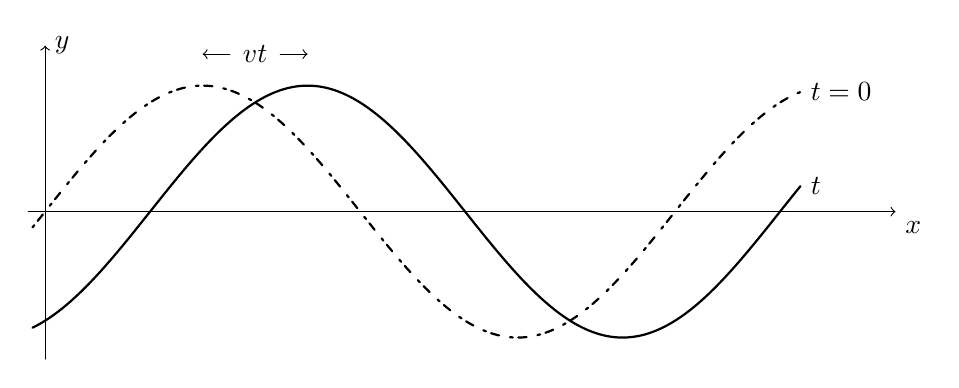
\begin{tikzpicture}[line cap=round,line join=round,x=8.0cm,y=8.0cm]
	%\draw[very thin,color=gray] (0,-0.24) grid (1.4,0.24);
	\draw[->,color=black] (-0.026820246306000255,0.) -- (1.35,0) node [anchor=north west] { $x$};
	%\foreach \x in {0.1,0.2,0.3,0.4,0.5,0.6,0.7,0.8,0.9,1.,1.1,1.2,1.3,1.4}
	%\draw[shift={(\x,0)},color=black] (0pt,2pt) -- (0pt,-2pt);
	%\draw[color=black] (1.4,0) node [anchor=north west] { $x$};
	\draw[->,color=black] (0.,-0.2341604564505571) -- (0.,0.2636169400770265) node [anchor=west] { $y$};
	%\foreach \y in {-0.2,-0.1,0.1,0.2}
	%\draw[shift={(0,\y)},color=black] (2pt,0pt) -- (-2pt,0pt);
	%\draw[color=black] (0.008952830872798266,0.22422448423671415) node [anchor = south west] { $y$};
	%\clip(-0.026820246306000255,-0.2341604564505571) rectangle (1.464721377102191,0.2636169400770265);
	\draw[line width=0.8pt,dash pattern=on 1pt off 2pt on 3pt off 4pt,smooth,samples=100,domain=-0.02:1.2] plot(\x,{0.2*sin((6.283185307179586*(\x)-6.283185307179586)*180/pi)}) node[right] {$t=0$};
	\draw[line width=0.8pt,smooth,samples=100,domain=-0.02:1.2] plot(\x,{0.2*sin((6.283185307179586*(\x)-6.283185307179586*(1.0+1/6))*180/pi)}) node[right] {$t$};
	%\draw (0.03943070215270692,2.6289548566703287) node[anchor= north west] {$y$};
	\draw[<-] (2/8,2/8) -- (2/8+1/12-0.04,2/8);
	\draw[->] (2/8+1/12+0.04,2/8) -- (2/8+1/6,2/8);
	\draw (1/3,2/8) node {$vt$};
	\end{tikzpicture}
	
	\caption{\emph{De uitwijking van een golf in functie van de tijd op $t=0$ en een willekeurig tijdstip $t$}}\label{afleiding_golfvergelijking}
	\end{figure}
	
	De verschijningsvorm van de golf in de ruimte kunnen we op $t=0$ weergeven met volgende sinusfunctie:
	\begin{eqnarray*}
	y=A\sin(kx)\qquad\mathrm{met}\qquad k=\frac{2\pi}{\lambda}
	\end{eqnarray*}
	Het symbool $k$ noemen we het \emph{golfgetal}.\footnote{De $k$ is eigenlijk niets anders dan de `$b$' zoals je die kent in de algemene sinusfunctie $f(x)=a\sin(b(x-c))$+d. $b=\frac{2\pi}{p}$ met $p$ de periode. In deze context is de periode de golflengte $\lambda$, uitgedrukt in meters.} \footnote{De $k$ heeft niets te maken met de veerconstante. Het is niet omdat Jantje Jantje heet en Jantje Jantje, dat Jantje en Jantje dezelfde personen zijn. Jantje en Jantje kunnen bijvoorbeeld -- al is het onwaarschijnlijk -- broers zijn.}
	\newline
	\newline
	Een tijd $t$ later is de verschijningsvorm van de golf een afstand $vt$ (de afstand die een top gedurende de tijd $t$ heeft afgelegd) naar rechts opgeschoven. De vergelijking vinden we dan door een overeenkomstige verschuiving door te voeren:
	\begin{eqnarray*}
	y&=&A\sin(k(x-vt))\\
	%&=&A\sin(kx-kvt)\\
	&=&A\sin\left(kx-\frac{2\pi v}{\lambda}t\right)\\
	&=&A\sin\left(kx-\frac{2\pi}{T}t\right)\\
	&=&A\sin\left(kx-\omega t\right)
	\end{eqnarray*}
	We hebben de uitwijking $y$ kunnen schrijven in functie van de variabelen $x$ en $t$. We hebben een algemene uitdrukking voor een rechtslopende golf:
	\begin{eqnarray}
	y(x,t)&=&A\sin\left(kx-\omega t\right)\label{rechtslopende_golf}
	\end{eqnarray}
	Om de vergelijking voor een linkslopende golf te vinden, verschuiven we naar links in plaats van naar rechts of vervangen we $v$ door $-v$. We krijgen dan
	\begin{eqnarray}
	y(x,t)&=&A\sin\left(kx+\omega t\right)\label{linkslopende_golf}
	\end{eqnarray}
	Deze functie in twee variabelen kunnen we iets beter verstaan wanneer we \'e\'en van de variabelen constant houden en de afhankelijkheid van de overblijvende variabele bekijken. Zo hebben we, wanneer we op een vaste plaats $x=x_0$ kijken, een harmonische trilling:
	\begin{eqnarray*}
	y_{x_0}(t)&=&y(x_0,t)=A\sin(\omega t+\underbrace{kx_0}_{\rm beginfase})
	\end{eqnarray*}
	Het is als het ware een patrijspoort van een stilstaand schip ter hoogte van de waterlijn. Een voorbijkomende golf is door het kleine venstertje slechts waar te nemen door het op- en neergaan van het waterniveau. Als we de tijd vastleggen door te kijken op \'e\'en bepaald tijdstip $t=t_0$, hebben we een functie die enkel de golf in de ruimte beschrijft.
	\begin{eqnarray*}
	y_{t_0}(x)&=&y(x,t_0)=A\sin(kx+\omega t_0)
	\end{eqnarray*}
	Het is alsof we een foto trekken van de golf.
	
	
	\newpage
	
	%\section{Verschijnselen}
	%
	%%\includepdf[pages={1},scale=1]{./golven_giancoli/scan_0.pdf}
	%
	%\begin{figure}[h]
	%\flushright
	%\includegraphics[width=0.8\textwidth]{./golven_giancoli/scan_0}
	%\end{figure}
	%
	%\begin{figure}[h]
	%\centering
	%\includegraphics[width=1.1\textwidth]{./golven_giancoli/scan_1}
	%\end{figure}
	%
	%\begin{figure}[h]
	%\centering
	%\includegraphics[width=1.1\textwidth]{./golven_giancoli/scan_2}
	%\end{figure}
	%
	%\begin{figure}[h]
	%\centering
	%\includegraphics[width=1.1\textwidth]{./golven_giancoli/scan_3}
	%\end{figure}
	%
	%\begin{figure}[h]
	%\centering
	%\includegraphics[width=1.1\textwidth]{./golven_giancoli/scan_4}
	%\end{figure}
	%
	%\begin{figure}[h]
	%\centering
	%\includegraphics[width=1.1\textwidth]{./golven_giancoli/scan_5}
	%\end{figure}
	%
	%\begin{figure}[h]
	%\centering
	%\includegraphics[width=1.1\textwidth]{./golven_giancoli/scan_6}
	%\end{figure}
	%
	%\begin{figure}[h]
	%\centering
	%\includegraphics[width=1.1\textwidth]{./golven_giancoli/scan_7}
	%\end{figure}
	%
	%\begin{figure}[h]
	%\centering
	%\includegraphics[width=1.1\textwidth]{./golven_giancoli/scan_8}
	%\end{figure}
	%
	%\begin{figure}[h]
	%\centering
	%\includegraphics[width=0.8\textwidth]{./golven_giancoli/scan_9}
	%\end{figure}
	%
	%\begin{figure}[h]
	%\centering
	%\includegraphics[width=0.8\textwidth]{./golven_giancoli/scan_10}
	%\end{figure}
	%
	%\begin{figure}[h]
	%\centering
	%\includegraphics[width=1.1\textwidth]{./golven_giancoli/scan_11}
	%\end{figure}
	%
	%%\begin{figure}[h]
	%%\centering
	%%\includegraphics[width=1.1\textwidth]{./golven_giancoli/scan_12}
	%%\end{figure}
	%
	%%\begin{figure}[h]
	%%\centering
	%%\includegraphics[width=1.1\textwidth]{./golven_giancoli/scan_13}
	%%\end{figure}
	%
	%%\subsection{Reflectie}
	%%vb echo, licht op een spiegel, zichtbare objecten
	%%
	%%\subsection{Breking/Refractie}
	%%
	%%overgang naar een andere middenstof. vb stok in water
	%%
	%%\subsection{Buiging/diffractie}
	%%om de hoek
	%%
	%%\subsection{Interferentie}
	%%
	%%- adhv watergolven/abstract?
	%%- twee fases? eerst gemakkelijk en vervolgens wiskundig?
	%%
	%%\section{Staande golven}
	%%
	%%\begin{tikzpicture}[domain=0:4] 
	%%    \draw[very thin,color=gray] (-0.1,-1.1) grid (3.9,3.9);
	%%    \draw[->] (-0.2,0) -- (4.2,0) node[right] {$x$}; 
	%%    \draw[->] (0,-1.2) -- (0,4.2) node[above] {$f(x)$};
	%%    \draw[color=red]    plot (\x,\x)             node[right] {$f(x) =x$}; 
	%%    \draw[color=blue]   plot (\x,{sin(\x r)})    node[right] {$f(x) = \sin x$}; 
	%%    \draw[color=orange] plot (\x,{0.05*exp(\x)}) node[right] {$f(x) = \frac{1}{20} \mathrm e^x$};
	%%  \end{tikzpicture}
	
	
\end{document}
